% Aberdeen style guide should be followed when using this
% layout. Their template powerpoint slide is used to extract the
% Aberdeen color and logo but is otherwise ignored (it has little or
% no formatting in it anyway).
%
% http://www.abdn.ac.uk/documents/style-guide.pdf

%%%%%%%%%%%%%%%%%%%% Document Class Settings %%%%%%%%%%%%%%%%%%%%%%%%%
% Pick if you want slides, or draft slides (no animations)
%%%%%%%%%%%%%%%%%%%%%%%%%%%%%%%%%%%%%%%%%%%%%%%%%%%%%%%%%%%%%%%%%%%%%%
%Normal document mode%
%\documentclass[10pt,compress,unknownkeysallowed]{beamer}
%Draft or handout mode
%\documentclass[10pt,compress,handout,unknownkeysallowed]{beamer}
\documentclass[10pt,compress,handout,ignorenonframetext,unknownkeysallowed]{beamer}

%%%%%%%%%%%%%%%%%%%% General Document settings %%%%%%%%%%%%%%%%%%%%%%%
% These settings must be set for each presentation
%%%%%%%%%%%%%%%%%%%%%%%%%%%%%%%%%%%%%%%%%%%%%%%%%%%%%%%%%%%%%%%%%%%%%%
\newcommand{\shortname}{jefferson.gomes@abdn.ac.uk}
\newcommand{\fullname}{Dr Jeff Gomes}
\institute{School of Engineering}
\newcommand{\emailaddress}{}%jefferson.gomes@abdn.ac.uk}
\newcommand{\logoimage}{../../FigBanner/UoAHorizBanner}
\title{Chemical Thermodynamics (EX3029)}
\subtitle{Module 4: Vapour-Liquid Equilibrium of Mixtures}
\date[ ]{ }

%%%%%%%%%%%%%%%%%%%% Template settings %%%%%%%%%%%%%%%%%%%%%%%%%%%%%%%
% You shouldn't have to change below this line, unless you want to.
%%%%%%%%%%%%%%%%%%%%%%%%%%%%%%%%%%%%%%%%%%%%%%%%%%%%%%%%%%%%%%%%%%%%%%
\usecolortheme{whale}
\useoutertheme{infolines}

% Use the fading effect for items that are covered on the current
% slide.
\beamertemplatetransparentcovered

% We abuse the author command to place all of the slide information on
% the title page.
\author[\shortname]{%
  \fullname\\\ttfamily{\emailaddress}
}


%At the start of every section, put a slide indicating the contents of the current section.
%\AtBeginSection[] {
%  \begin{frame}
%    \frametitle{Section Outline}
%    \tableofcontents[currentsection]
%  \end{frame}
%}

% Allow the inclusion of movies into the Presentation! At present,
% only the Okular program is capable of playing the movies *IN* the
% presentation.
\usepackage{multimedia}
\usepackage{animate}

%% Handsout -- comment out the lines below to create handstout with 4 slides in a page with space for comments
\usepackage{handoutWithNotes}

\mode<handout>
{
\usepackage{pgf,pgfpages}

\pgfpagesdeclarelayout{2 on 1 boxed with notes}
{
\edef\pgfpageoptionheight{\the\paperheight} 
\edef\pgfpageoptionwidth{\the\paperwidth}
\edef\pgfpageoptionborder{0pt}
}
{
\setkeys{pgfpagesuselayoutoption}{landscape}
\pgfpagesphysicalpageoptions
    {%
        logical pages=4,%
        physical height=\pgfpageoptionheight,%
        physical width=\pgfpageoptionwidth,%
        last logical shipout=2%
    } 
\pgfpageslogicalpageoptions{1}
    {%
    border code=\pgfsetlinewidth{1pt}\pgfstroke,%
    scale=1,
    center=\pgfpoint{.25\pgfphysicalwidth}{.75\pgfphysicalheight}%
    }%
\pgfpageslogicalpageoptions{2}
    {%
    border code=\pgfsetlinewidth{1pt}\pgfstroke,%
    scale=1,
    center=\pgfpoint{.25\pgfphysicalwidth}{.25\pgfphysicalheight}%
    }%
\pgfpageslogicalpageoptions{3}
    {%
    border shrink=\pgfpageoptionborder,%
    resized width=.7\pgfphysicalwidth,%
    resized height=.5\pgfphysicalheight,%
    center=\pgfpoint{.75\pgfphysicalwidth}{.29\pgfphysicalheight},%
    copy from=3
    }%
\pgfpageslogicalpageoptions{4}
    {%
    border shrink=\pgfpageoptionborder,%
    resized width=.7\pgfphysicalwidth,%
    resized height=.5\pgfphysicalheight,%
    center=\pgfpoint{.75\pgfphysicalwidth}{.79\pgfphysicalheight},%
    copy from=4
    }%

\AtBeginDocument
    {
    \newbox\notesbox
    \setbox\notesbox=\vbox
        {
            \hsize=\paperwidth
            \vskip-1in\hskip-1in\vbox
            {
                \vskip1cm
                Notes\vskip1cm
                        \hrule width\paperwidth\vskip1cm
                    \hrule width\paperwidth\vskip1cm
                        \hrule width\paperwidth\vskip1cm
                    \hrule width\paperwidth\vskip1cm
                        \hrule width\paperwidth\vskip1cm
                    \hrule width\paperwidth\vskip1cm
                    \hrule width\paperwidth\vskip1cm
                    \hrule width\paperwidth\vskip1cm
                        \hrule width\paperwidth
            }
        }
        \pgfpagesshipoutlogicalpage{3}\copy\notesbox
        \pgfpagesshipoutlogicalpage{4}\copy\notesbox
    }
}
}

%\pgfpagesuselayout{2 on 1 boxed with notes}[letterpaper,border shrink=5mm]

%%%%% Color settings
\usepackage{color}
%% The background color for code listings (i.e. example programs)
\definecolor{lbcolor}{rgb}{0.9,0.9,0.9}%
\definecolor{UoARed}{rgb}{0.64706, 0.0, 0.12941}
\definecolor{UoALight}{rgb}{0.85, 0.85, 0.85}
\definecolor{UoALighter}{rgb}{0.92, 0.92, 0.92}
\setbeamercolor{structure}{fg=UoARed} % General background and higlight color
\setbeamercolor{frametitle}{bg=black} % General color
\setbeamercolor{frametitle right}{bg=black} % General color
\setbeamercolor{block body}{bg=UoALighter} % For blocks
\setbeamercolor{structure}{bg=UoALight} % For blocks
% Rounded boxes for blocks
\setbeamertemplate{blocks}[rounded]

%%%%% Font settings
% Aberdeen requires the use of Arial in slides. We can use the
% Helvetica font as its widely available like so
% \usepackage{helvet}
% \renewcommand{\familydefault}{\sfdefault}
% But beamer already uses a sans font, so we will stick with that.

% The size of the font used for the code listings.
\newcommand{\goodsize}{\fontsize{6}{7}\selectfont}

% Extra math packages, symbols and colors. If you're using Latex you
% must be using it for formatting the math!
\usepackage{amscd,amssymb} \usepackage{amsfonts}
\usepackage[mathscr]{eucal} \usepackage{mathrsfs}
\usepackage{latexsym} \usepackage{amsmath} \usepackage{bm}
\usepackage{amsthm} \usepackage{textcomp} \usepackage{eurosym}
% This package provides \cancel{a} and \cancelto{a}{b} to "cancel"
% expressions in math.
\usepackage{cancel}

\usepackage{comment} 

% Get rid of font warnings as modern LaTaX installations have scalable
% fonts
\usepackage{type1cm} 

%\usepackage{enumitem} % continuous numbering throughout enumerate commands

% For exact placement of images/text on the cover page
\usepackage[absolute]{textpos}
\setlength{\TPHorizModule}{1mm}%sets the textpos unit
\setlength{\TPVertModule}{\TPHorizModule} 

% Source code formatting package
\usepackage{listings}%
\lstset{ backgroundcolor=\color{lbcolor}, tabsize=4,
  numberstyle=\tiny, rulecolor=, language=C++, basicstyle=\goodsize,
  upquote=true, aboveskip={1.5\baselineskip}, columns=fixed,
  showstringspaces=false, extendedchars=true, breaklines=false,
  prebreak = \raisebox{0ex}[0ex][0ex]{\ensuremath{\hookleftarrow}},
  frame=single, showtabs=false, showspaces=false,
  showstringspaces=false, identifierstyle=\ttfamily,
  keywordstyle=\color[rgb]{0,0,1},
  commentstyle=\color[rgb]{0.133,0.545,0.133},
  stringstyle=\color[rgb]{0.627,0.126,0.941}}

% Allows the inclusion of other PDF's into the final PDF. Great for
% attaching tutorial sheets etc.
\usepackage{pdfpages}
\setbeamercolor{background canvas}{bg=}  

% Remove foot note horizontal rules, they occupy too much space on the slide
\renewcommand{\footnoterule}{}

% Force the driver to fix the colors on PDF's which include mixed
% colorspaces and transparency.
\pdfpageattr {/Group << /S /Transparency /I true /CS /DeviceRGB>>}

% Include a graphics, reserve space for it but
% show it on the next frame.
% Parameters:
% #1 Which slide you want it on
% #2 Previous slides
% #3 Options to \includegraphics (optional)
% #4 Name of graphic
\newcommand{\reserveandshow}[4]{%
\phantom{\includegraphics<#2|handout:0>[#3]{#4}}%
\includegraphics<#1>[#3]{#4}%
}

\newcommand{\frc}{\displaystyle\frac}
\newcommand{\red}{\textcolor{red}}
\newcommand{\blue}{\textcolor{blue}}
\newcommand{\green}{\textcolor{green}}
\newcommand{\purple}{\textcolor{purple}}
\newcommand{\summation}[3][error]{\sum\limits_{#2}^{#3}#1}
 
\begin{document}

% Title page layout
\begin{frame}
  \titlepage
  \vfill%
  \begin{center}
    \includegraphics[clip,width=0.8\textwidth]{\logoimage}
  \end{center}
\end{frame}

% Table of contents
\frame{ \frametitle{Slides Outline}
  \tableofcontents
}


%%%%%%%%%%%%%%%%%%%% The Presentation Proper %%%%%%%%%%%%%%%%%%%%%%%%%
% Fill below this line with \begin{frame} commands! It's best to
% always add the fragile option incase you're going to use the
% verbatim environment.
%%%%%%%%%%%%%%%%%%%%%%%%%%%%%%%%%%%%%%%%%%%%%%%%%%%%%%%%%%%%%%%%%%%%%%

%%%
%%% SECTION
%%%
\section{General Remarks}

%%%
%%% Slides
%%%
\begin{frame}
 \frametitle{Aims and Objectives}
   \begin{enumerate}
     \item<1-> In Modules 2-3, we focused on 
       \begin{enumerate}
         \item<1-> Evaluating partial derivatives of thermodynamic variables and derive fundamental thermodynamic relations;
         \item<1-> Obtaining volumetric EOS parameters from critical properties;
         \item<1-> Studying thermodynamic behaviour of pure substances in arbitrary number of phases (multiphase).
       \end{enumerate} 
     \item<2-> However, in most industrial processes more than one chemical specie is present within multiple phases in thermodynamic equilibrium. 
     \item<3-> Our focus in this Module is to study equilibrium of arbitrary number of chemical species at vapour and liquid phases.
     \item<4-> This Module focuses on 
         \begin{enumerate}
           \item<4-> Partial molar properties; 
           \item<4-> Vapour-liquid equilibrium (VLE) relations and the main diagrams ($x-y$, $T-xy$ and $P-xy$); 
           %\item<4-> Concept of activity, fugacity, chemical potential (and its relationship with the free Gibbs energy).
         \end{enumerate}
   \end{enumerate}
\end{frame}


%%%
%%% SECTION
%%%
\subsection{Bibliography}
\begin{frame}
 \frametitle{Suggested References}
  Literature relevant for this module:
  \begin{enumerate}[(i)]
   \item\label{SVN_Book} J.M. Smith, H.C. Van Ness, M.M. Abbott, $\lq$Introduction to Chemical Engineering Thermodynamics', 6$^{th}$ Edition: Chapter 10;
   \item Y.V.C. Rao, $\lq$Chemical Engineering Thermodynamics',4$^{th}$ Edition: Chapters 10 and 12.
   \item\label{Sandle_Book} S.I. Sandler, $\lq$Chemical, Biochemical and Engineering Thermodynamics', 4$^{th}$ Edition: Chapter 10.
  \end{enumerate}
\end{frame}


%%%
%%% SUBSECTION
%%%
\subsection{Introduction} 

%%%
%%% Slide
%%%
%\scriptsize
\begin{frame}
  \frametitle{Introduction}
  \begin{enumerate}
    \item<1-> In most technical processes there are no pure substances but a mixture of various species in
        \begin{enumerate}
          \item<1-> industrial reactors and pressure vessels $\&$ tanks;
          \item<1-> separation process facilities (e.g., distillation, absorption, extraction etc);
          \item<1-> subsurface transport processes (e.g., groundwater pollutant contamination, hydrocarbon exploration etc).     
        \end{enumerate}
    \item<2-> It is necessary \textcolor{blue}{to identify how the concentration of species will change during the process};
    \item<3-> During \textcolor{blue}{phase equilibrium} we need to be able to effectively quantify variations in the thermodynamic properties, \textcolor{blue}{in particular, concentration}. This quantitative analysis is crucial in the design of processes and equipment;
    \item<4-> \textcolor{blue}{Equilibria} of industrial interest:
        \begin{enumerate}
          \item<5-> \textcolor{blue}{Vapour-Liquid (VLE)}: distillation;
          \item<5-> Liquid-Liquid (LLE): extraction;
          \item<5-> Solid-vapour (SVE): particle generation;
          \item<5-> Liquid-solid (LSE): cristallisation
        \end{enumerate}
    \item<5-> {\it In this Module we will only consider non-reacting systems.}
  \end{enumerate}
\end{frame}
\normalsize


%%%
%%% Slide
%%%
%\scriptsize
\begin{frame}
  \frametitle{Representing Composition}
  \begin{enumerate}
    \item<1-> Molar fraction $\left(x_{i}\right)$:
         \visible<1->{\begin{displaymath}
            %w_{i} = \frc{m_{i}}{m} = \frc{\dot{m}_{i}}{\dot{m}} \;\;\;\text{ and }\;\;\; x_{i} = \frc{n_{i}}{n} = \frc{\dot{n}_{i}}{\dot{n}}
            x_{i} = \frc{n_{i}}{n} 
         \end{displaymath}}
         where $n = n_{1}+\cdots+n_{\mathcal{C}} = \summation[n_{i}]{i=1}{\mathcal{C}}$.
         %where $\left[\dot{\gamma}\right]$ represents flow rate quantities.}
    \item<2-> Molar concentration:
         \visible<2->{\begin{displaymath}
            C_{i} = \frc{n_{i}}{V} 
         \end{displaymath}
          also called \textcolor{blue}{molarity}.}
   % \item<2-> Molar concentration in flow process:
   %      \visible<2->{\begin{displaymath}
   %         C_{i} = \frc{\dot{n}_{i}}{\dot{q}} 
   %      \end{displaymath}
   %      where $\dot{q}$ is the volumetric flow rate.}
    \item<3-> (Average) Molar mass of mixtures:
         \visible<3->{\begin{displaymath}
            \overline{MW} = \sum\limits_{i} \left(x_{i} \cdot MW_{i}\right) 
         \end{displaymath}
         where $MW_{i}$ is the molecular weight (or molar mass) of species $i$.}
  \end{enumerate}
\end{frame}
\normalsize


\subsection{Excess Properties}
%%%
%%% Slide
%%%
%\scriptsize
\begin{frame}
  \frametitle{Excess Properties}
  \visible<1->{\begin{block}{Excess Mixing Properties (Sandler)}
$\lq$\textcolor{blue}{Excess mixing property} is the change in the extensive thermodynamic property $M$ that occurs on mixing at constant pressure and temperature in addition to that which would occur if an ideal mixture were formed.'
  \end{block}}
  \visible<1->{\begin{displaymath}
     M^{\text{E}} = M - M^{\text{id}}
  \end{displaymath}
  $M$ is the actual property of the mixture, and $M^{\text{id}}$ is the ideal solution property.}\\
  \visible<2->{This accounts for extensive properties of the individual components, i.e.,
     \begin{displaymath}
     M^{\text{id}} = \sum\limits_{i} x_{i} M_{i}
  \end{displaymath}}
  \medskip\noindent
  \visible<3->{For two components,
      \begin{displaymath}
         \textcolor{blue}{V^{\text{E}}} = V - V^{\text{id}} = V - \sum\limits_{i} x_{i} V_{i} = \textcolor{blue}{V - \left(x_{1}V_{1} + x_{2}V_{2}\right)}
      \end{displaymath}} 
\end{frame}
\normalsize

%%%
%%% SECTION
%%%
\section{Equilibrium Conditions}

\subsection{Stability Test}
%%%
%%% Slide
%%%
%\scriptsize
\begin{frame}
  \frametitle{Equilibrium Conditions and Stability Criteria}
     \begin{center}
         \begin{tabular}{l l l c}
         \hline\hline
            {\bf System}         &   {\bf Constraint}    &    {\bf Equilibrium}            & {\bf Stability } \\
                                 &                       &    {\bf Criterion}              & {\bf Criterion} \\ 
         \hline
            Isolated, adiabatic  &  $U$ and $V$          &      $S$ = maximum               &    d$^{2}$S$<$ 0    \\
            fixed-boundary system&   constant            &      $dS$ = 0                    &                     \\
         \hline
            Isothermal closed    &   $T$ and $V$         &      $A$ = minimum               &                   \\
            system with fixed    &   constant            &      $dA$ = 0                    &  d$^{2}$A $>$ 0    \\
            boundaries           &                       &                                  &                    \\
         \hline
            Isothermal, isobaric &  $T$ and $P$          &    $G$ = minimum                 &  d$^{2}$G $>$ 0    \\
            closed system        &   constant            &    $dG$ = 0                      &                    \\
         \hline
            Isothermal, isobaric &  $T$, $P$ and $N$    &     $G$ = minimum                 &   \\
            open system moving  with& constant          &     $dG$ = 0                      & d$^{2}$G $>$ 0    \\
           the fluid velocity    &                      &                                   &                   \\
         \hline\hline
         \end{tabular}
     \end{center}
   \end{frame}
\normalsize

%%%
%%% SECTION
%%%
\section{Vapour-Liquid Equilibrium (VLE)}

\subsection{Qualitative Behaviour}
%%%
%%% Slide
%%%
%\scriptsize
\begin{frame}
  \frametitle{$P$-$T$-$xy$ Diagram}
  \begin{columns}
     \begin{column}[l]{0.3\linewidth}
        \begin{enumerate}
            \item<1-> System with $\mathcal{C} =2$ (hexane and triethylamine, extracted from Sandler, 2006);
            \item<2-> From the phase rule: $\Psi = 4 -\mathcal{P}$;
                \begin{enumerate}
                    \item<3-> For $\mathcal{P}=1$ $\Longrightarrow$ $\Psi=3$, i.e., $P$, $T$ and {\bf one} mole fraction;
                    \item<4-> For $\mathcal{P}=2$ $\Longrightarrow$ $\Psi=2$ $\leftrightarrow$ define surfaces;
                \end{enumerate}
            \item<5-> \textcolor{blue}{Surfaces} represent equilibrium states: saturated vapour and liquid.
        \end{enumerate}
     \end{column}
     \begin{column}[l]{0.7\linewidth}
        \hbox{\hspace{-1cm}
           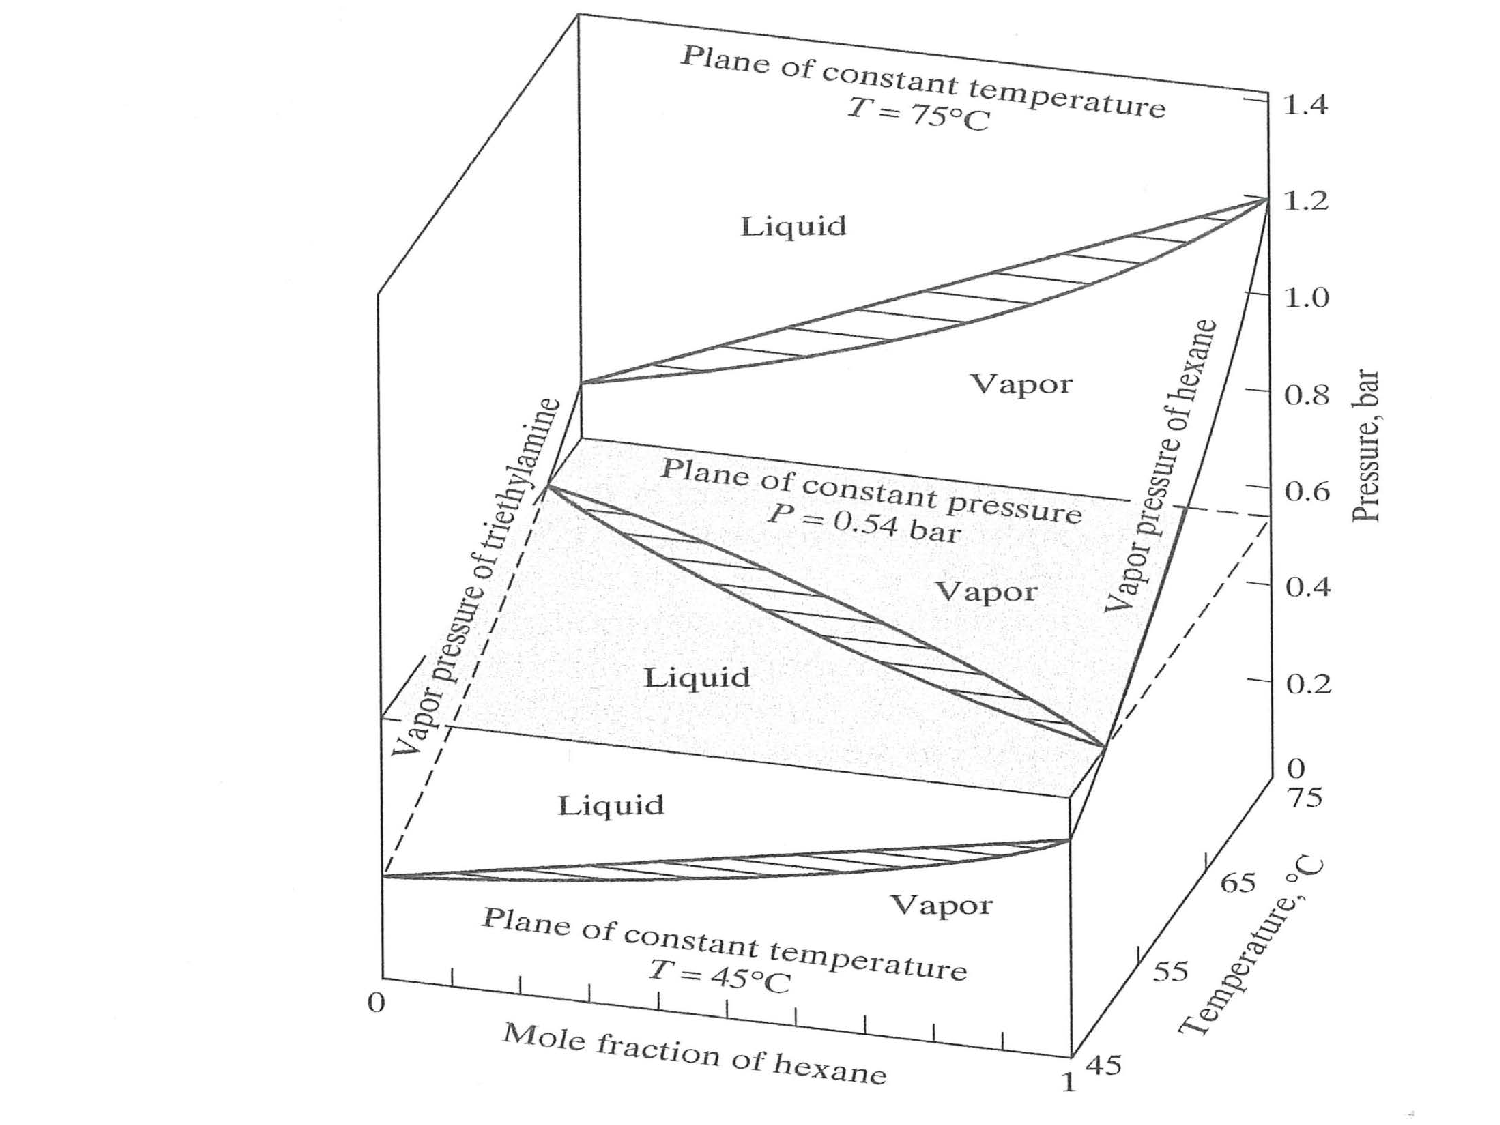
\includegraphics[width=9.7cm,clip]{./../Pics/PTxy_diagram}}
     \end{column}
  \end{columns}
\end{frame}
\normalsize

%%%
%%% Slide
%%%
%\scriptsize
\begin{frame}
  \frametitle{$P$-$T$-$xy$ Diagram}
     \begin{center}
       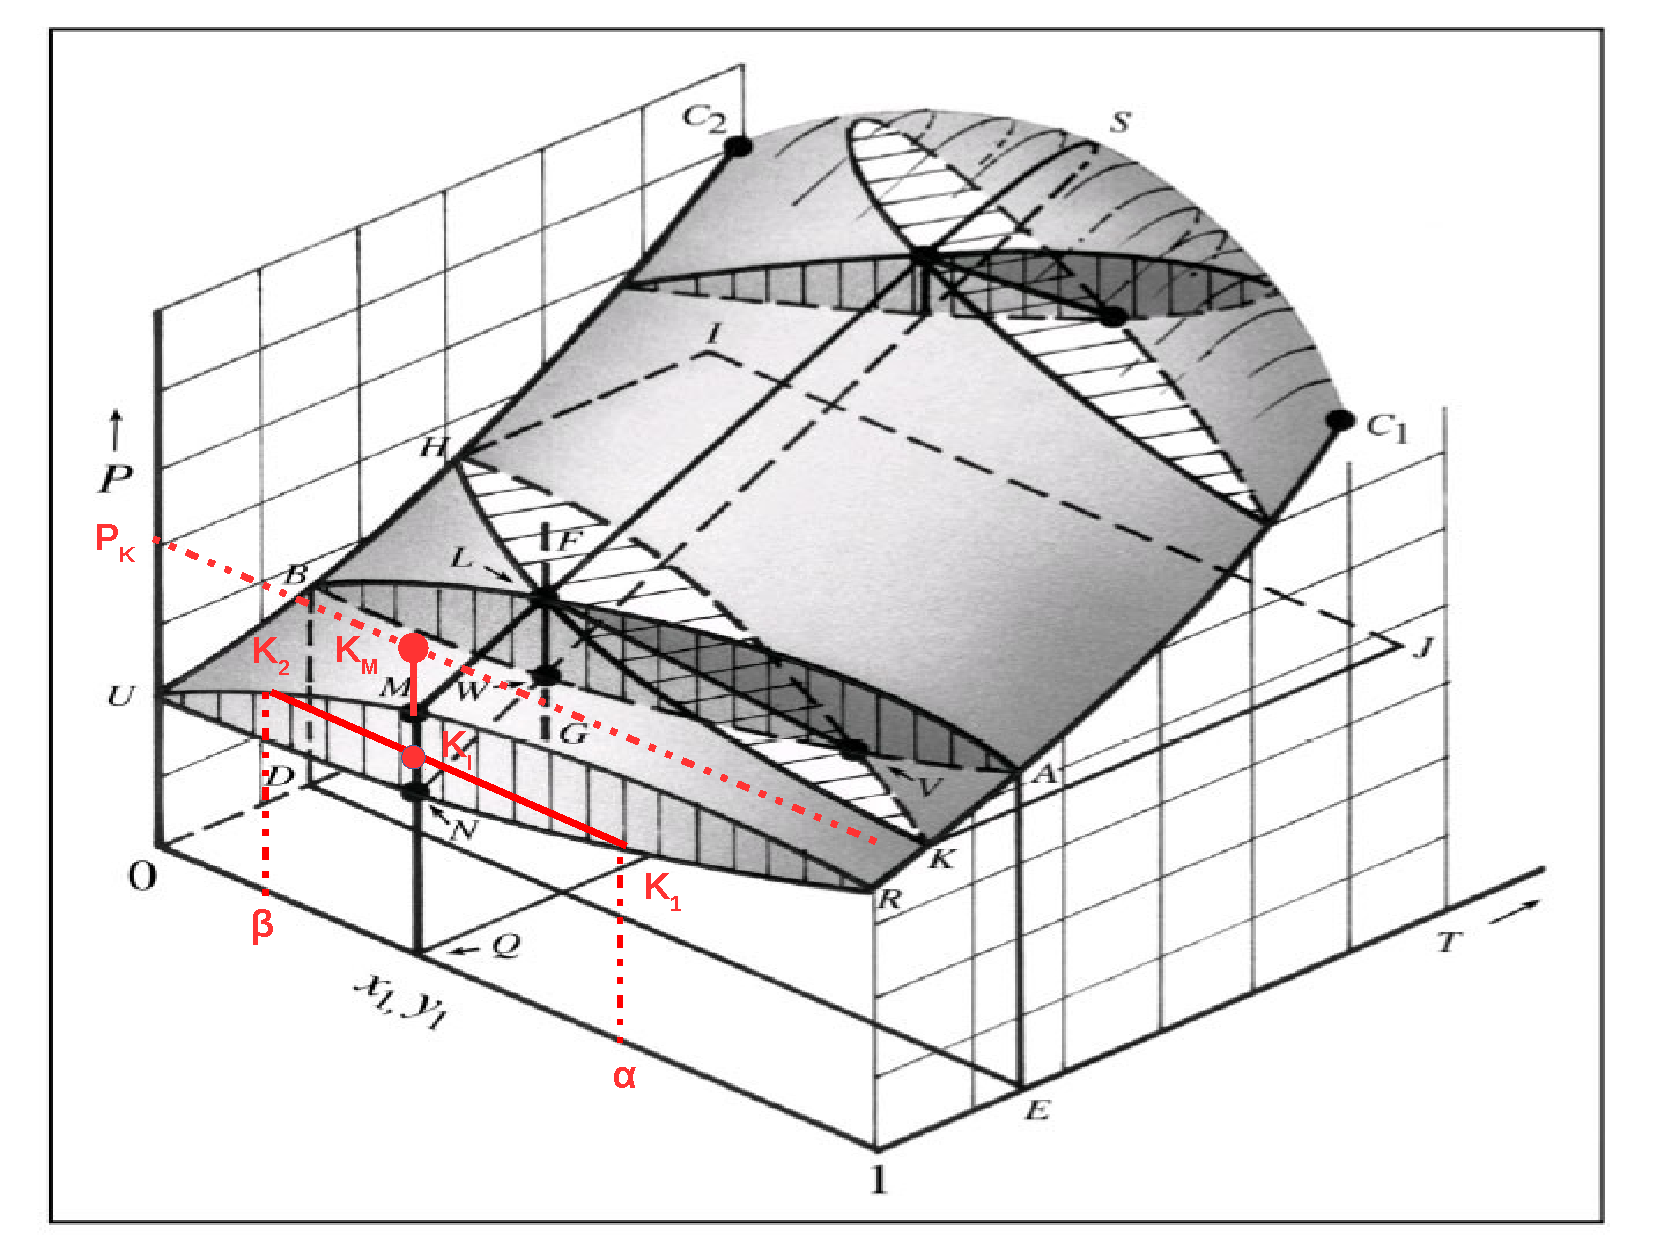
\includegraphics[width=.75\columnwidth,clip]{./Figs/PTxy_Digram} %{./../Pics/PTxy_diagram2}
     \end{center}
\end{frame}
\normalsize



%%%
%%% Slide
%%%
%\scriptsize
\begin{frame}
  \frametitle{$P-T$ Diagrams at fixed composition}
  \begin{columns}
     \begin{column}[l]{0.5\linewidth}
        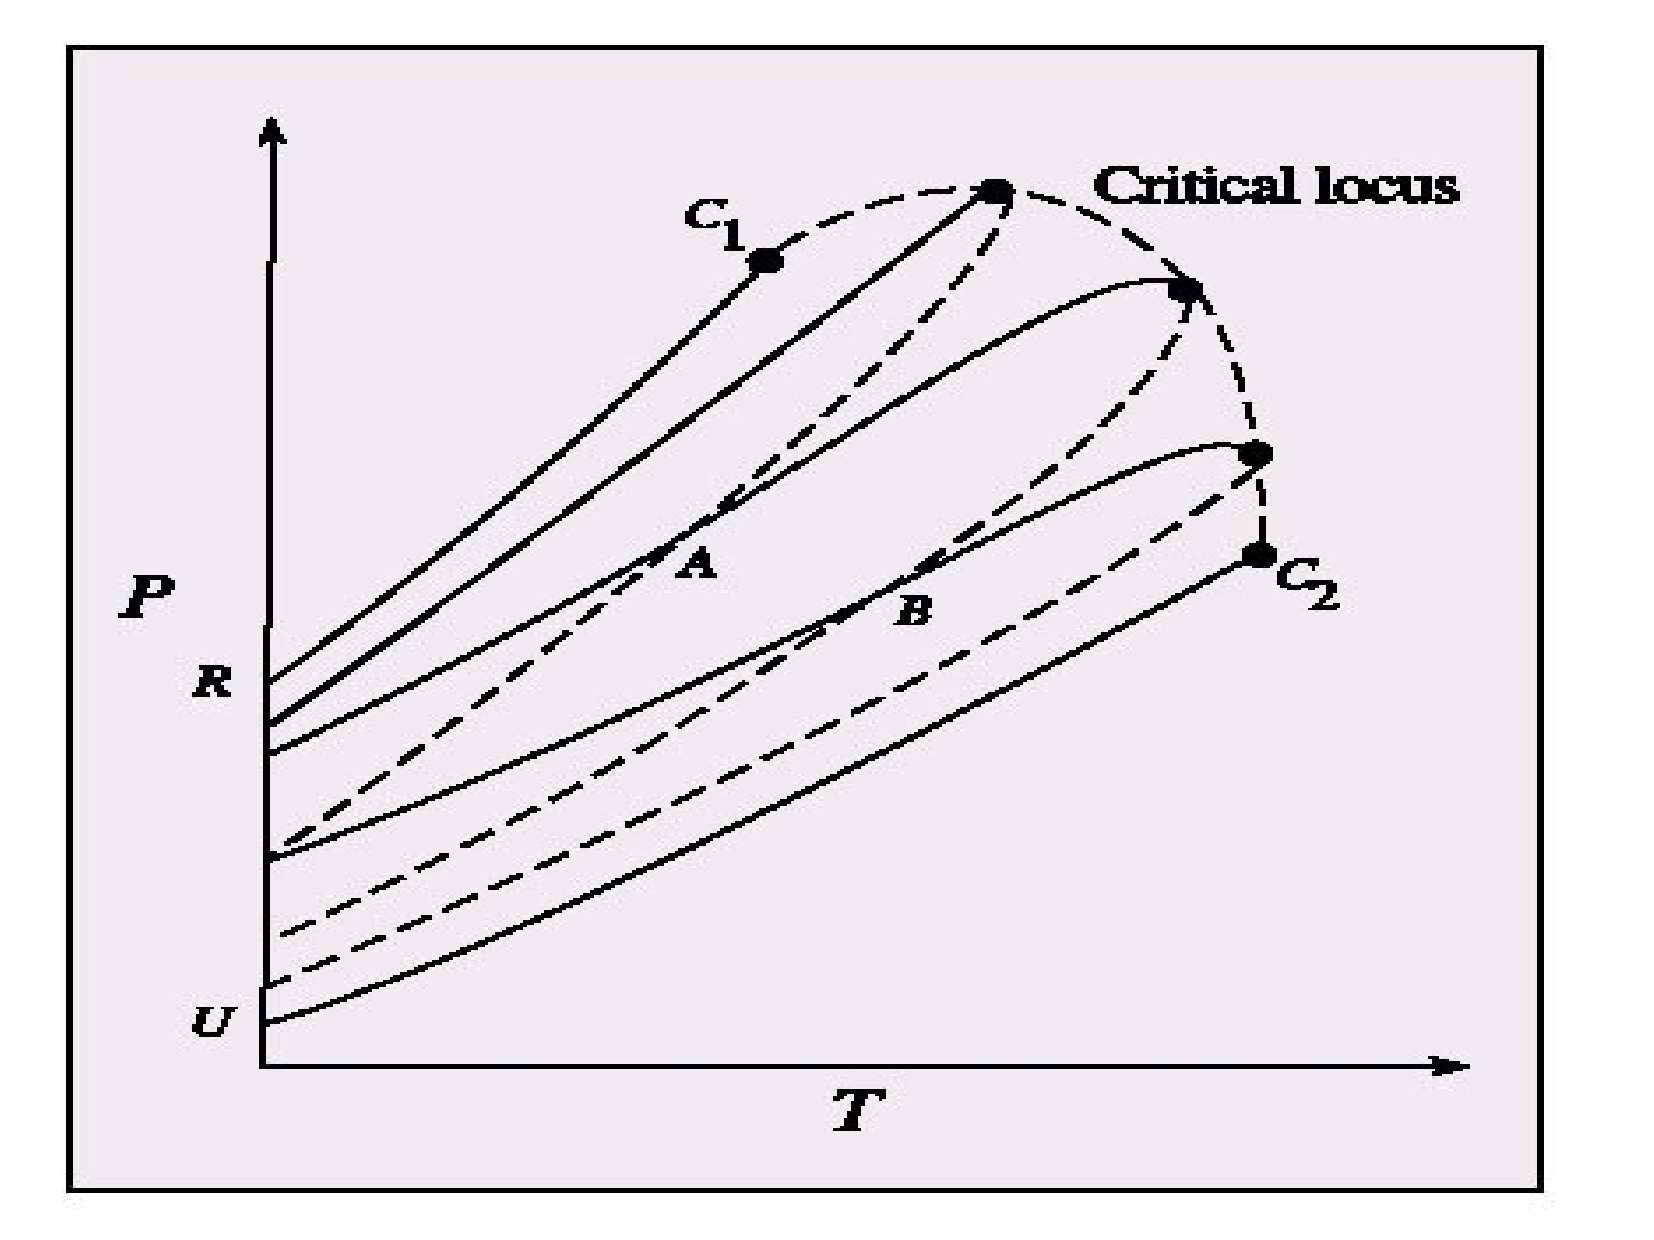
\includegraphics[width=\linewidth,clip]{./../Pics/VLE_PT_diagram1}
     \end{column}
     \begin{column}[l]{0.5\linewidth}
        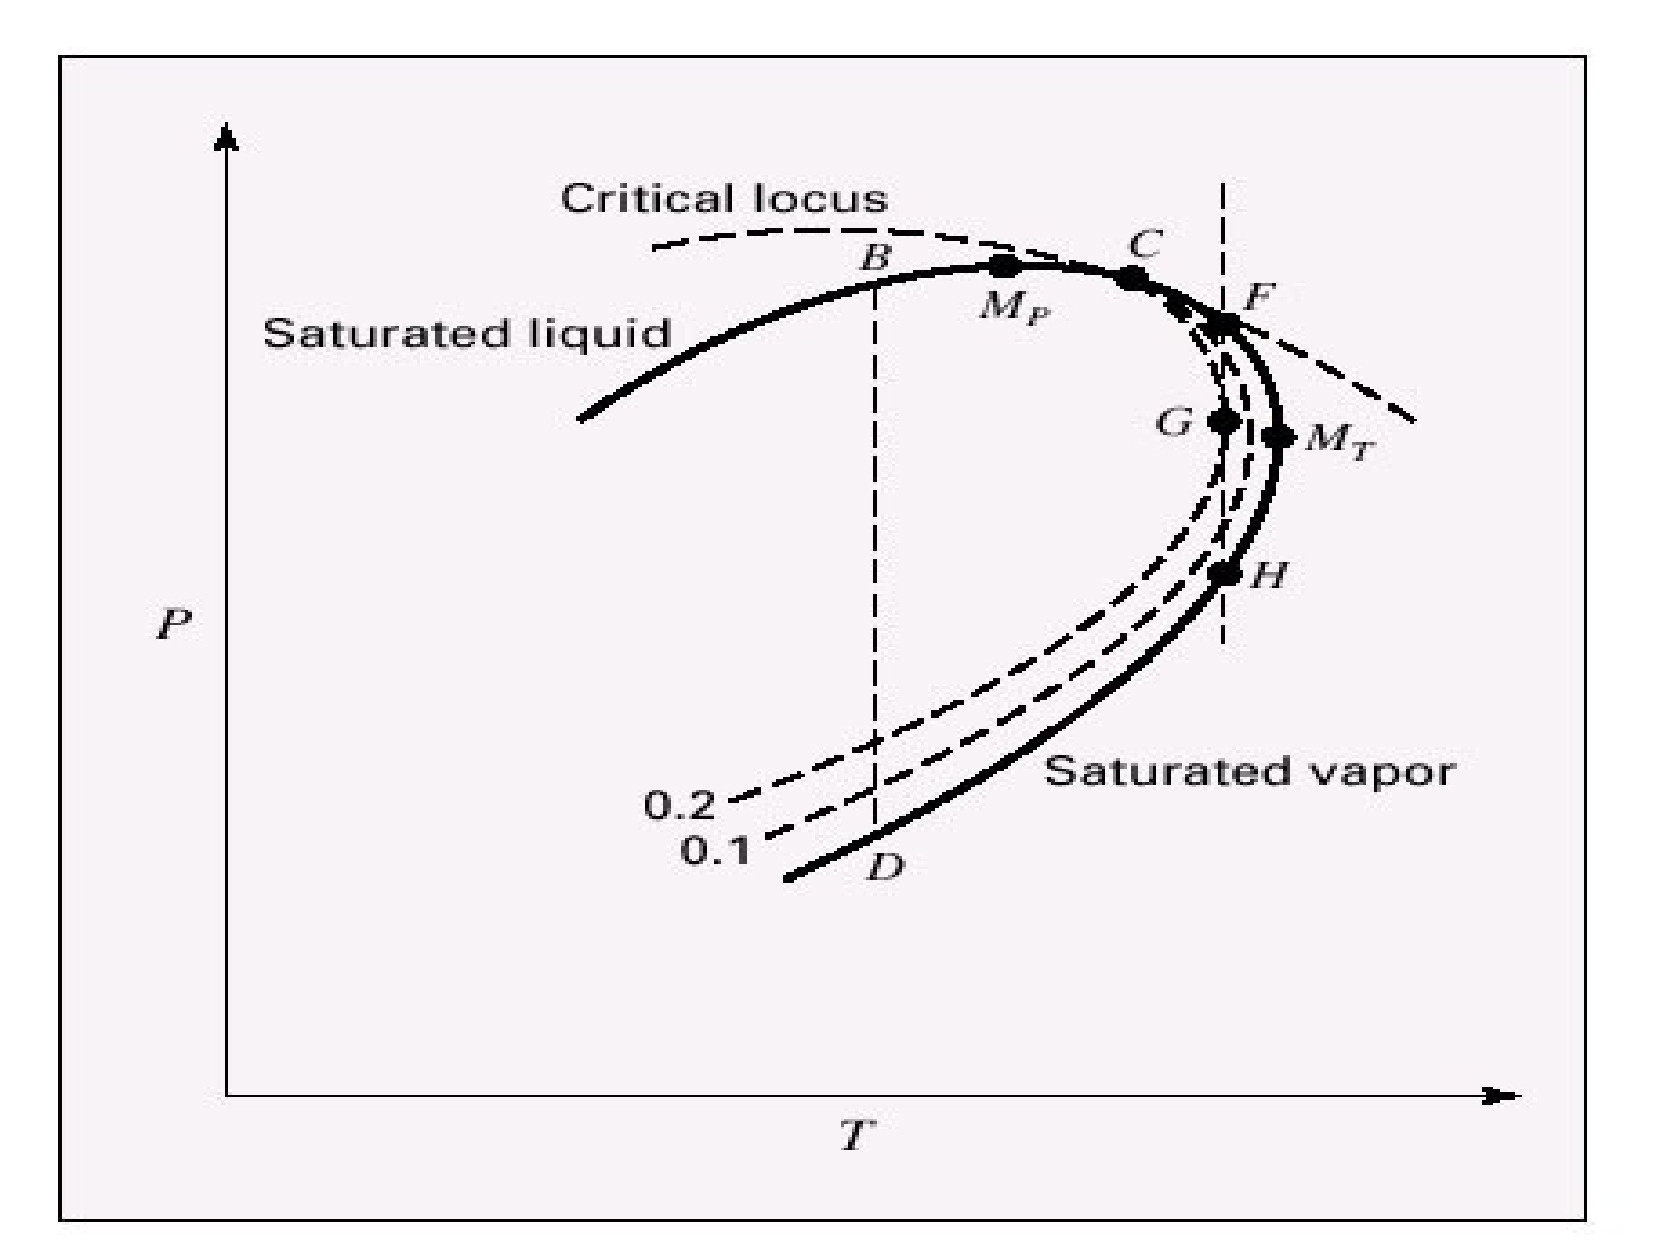
\includegraphics[width=\linewidth,clip]{./../Pics/VLE_PT_diagram2}
     \end{column}
  \end{columns}
  \begin{center}
     Solid line: saturated liquid (bubble line); \\
     Dashed line: saturated vapour (dew line) 
  \end{center}
\end{frame}
\normalsize


%%%
%%% Slide
%%%
\scriptsize
\begin{frame}
  \frametitle{$Pxy$ Diagrams} 
  \vspace{-0.8cm}
  \begin{columns}
     \begin{column}[l]{0.5\linewidth}
        \visible<1->{\hbox{\hspace{-1.7cm}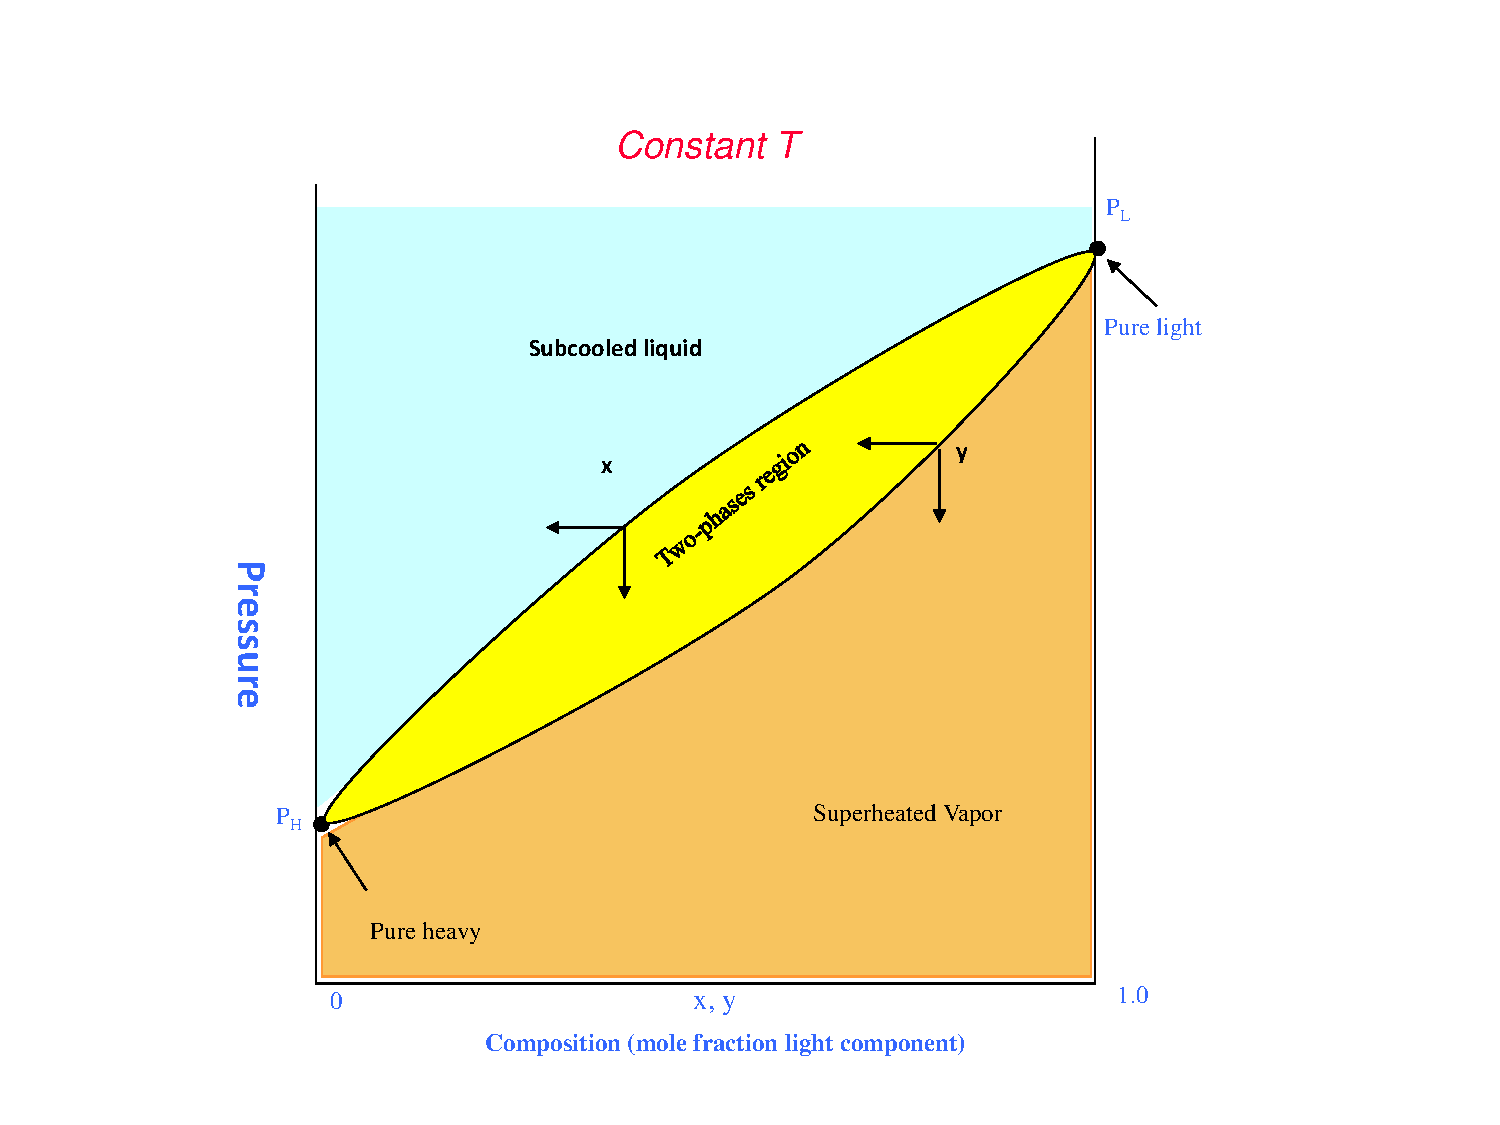
\includegraphics[width=1.6\linewidth,clip]{./../Pics/VLE_Pxy_Diagram1}}}
        %Upper curve: liquid phase composition $x$;\\
        %Lower curve: vapour phase composition $y$;
     \end{column}
     \begin{column}[l]{0.5\linewidth}
       \visible<2->{\hbox{\hspace{-1.7cm}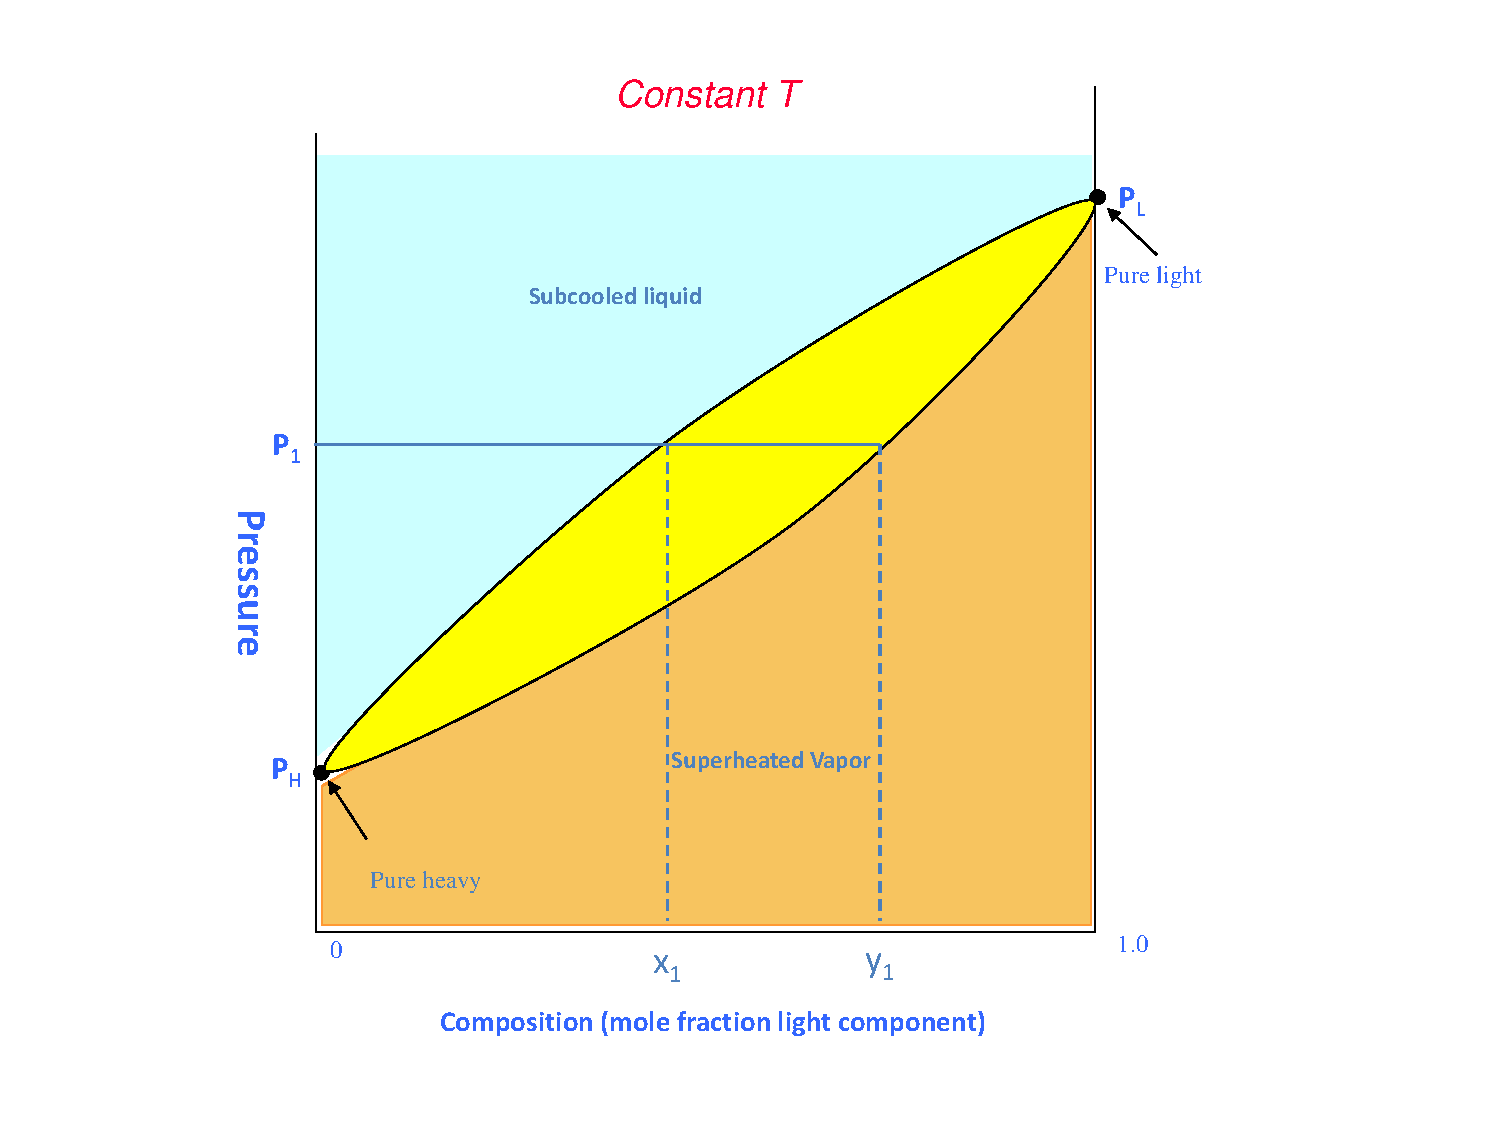
\includegraphics[width=1.6\linewidth,clip]{./../Pics/VLE_Pxy_Diagram2}}}
     \end{column}
  \end{columns}
         \visible<1->{Upper and lower curves represent liquid ($x$) and vapour phases compositions.}\\
         \visible<2->{$P_{H}$ and $P_{L}$ are the vapour pressure of pure heavy and light components at temperature $T$, respectively.}
\end{frame}
\normalsize


%%%
%%% Slide
%%%
%\scriptsize
\begin{frame}
  \frametitle{$Pxy$ Diagrams}
  \begin{columns}
     \begin{column}[l]{0.5\linewidth}
       \begin{enumerate}
          \item<1-> For a given \textcolor{blue}{initial (feed) composition $z$} (at constant $T$), if pressure is raised to $P_{\text{DP}}$, the first droplet of liquid is formed. \textcolor{blue}{$P_{\text{DB}}$} is called {\bf \textcolor{blue}{dew point}};
          \item<2-> The liquid droplets are much leaner in the light component and the composition is ${\bf \textcolor{blue}{x_{\text{DB}}}}$;
          \item<3-> As the pressure is further increased, more liquid is formed. At \textcolor{blue}{P$_{1}$}, liquid and vapour are in equilibrium with composition $\textcolor{blue}{x_{1}}$ and $\textcolor{blue}{y_{1}}$;
          \item<4-> When the pressure reaches \textcolor{blue}{P$_{\text{BP}}$}, the last bubble of vapour condenses -- {\bf \textcolor{blue}{bubble point}}.  
       \end{enumerate}
     \end{column}
     \begin{column}[l]{0.5\linewidth}
        \visible<1->{\hbox{\hspace{.0cm}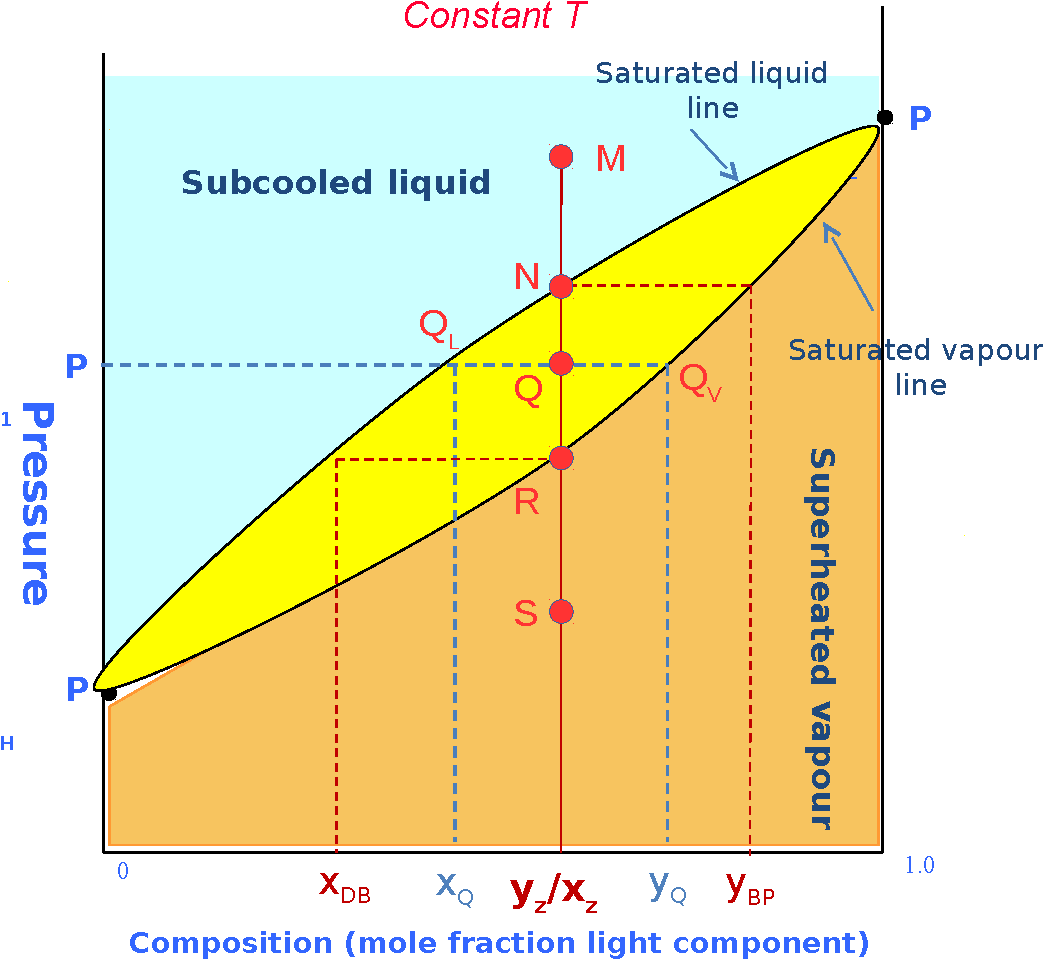
\includegraphics[width=1.\linewidth,clip]{./../Pics/VLE_Pxy_Diagram3b}}}
     \end{column}
  \end{columns}
\end{frame}
\normalsize


%%%
%%% Slide
%%%
%\scriptsize
\begin{frame}
  \frametitle{$xy$ Diagrams}
  \begin{columns}
     \begin{column}[l]{0.4\linewidth}
       \begin{enumerate}
          \item<1-> The $xy$ diagram for a binary system correlates the compositions of the liquid and vapour phases in equilibrium;
          \item<1-> They are designed assuming either constant $P$ or $T$ $\Longrightarrow$ though most industrial applications are isobaric.
       \end{enumerate}
     \end{column}
     \begin{column}[l]{0.6\linewidth}
        \visible<1->{\hbox{\hspace{-.0cm}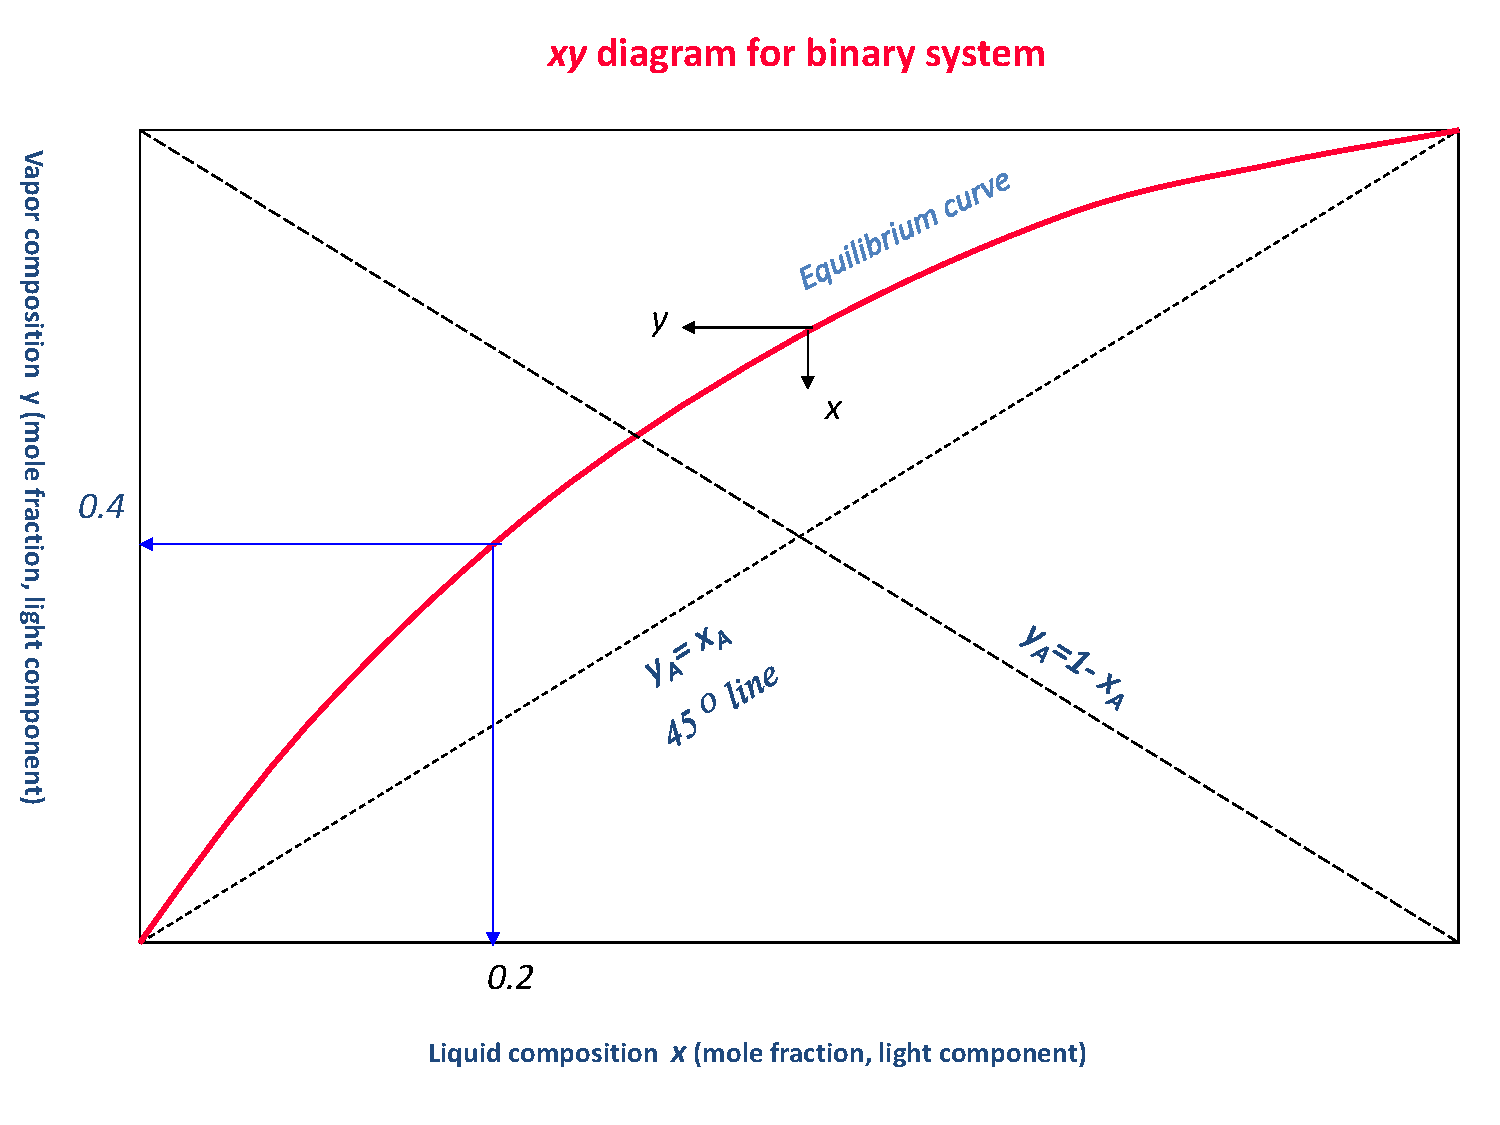
\includegraphics[width=1.\linewidth,clip]{./../Pics/VLE_xy_Diagram1}}}
     \end{column}
  \end{columns}
\end{frame}
\normalsize


%%%
%%% Slide
%%%
%\scriptsize
\begin{frame}
  \frametitle{$xy$ Diagrams: Ideal and Non-Ideal Solutions}
  \vbox{
     \hbox{\visible<1->{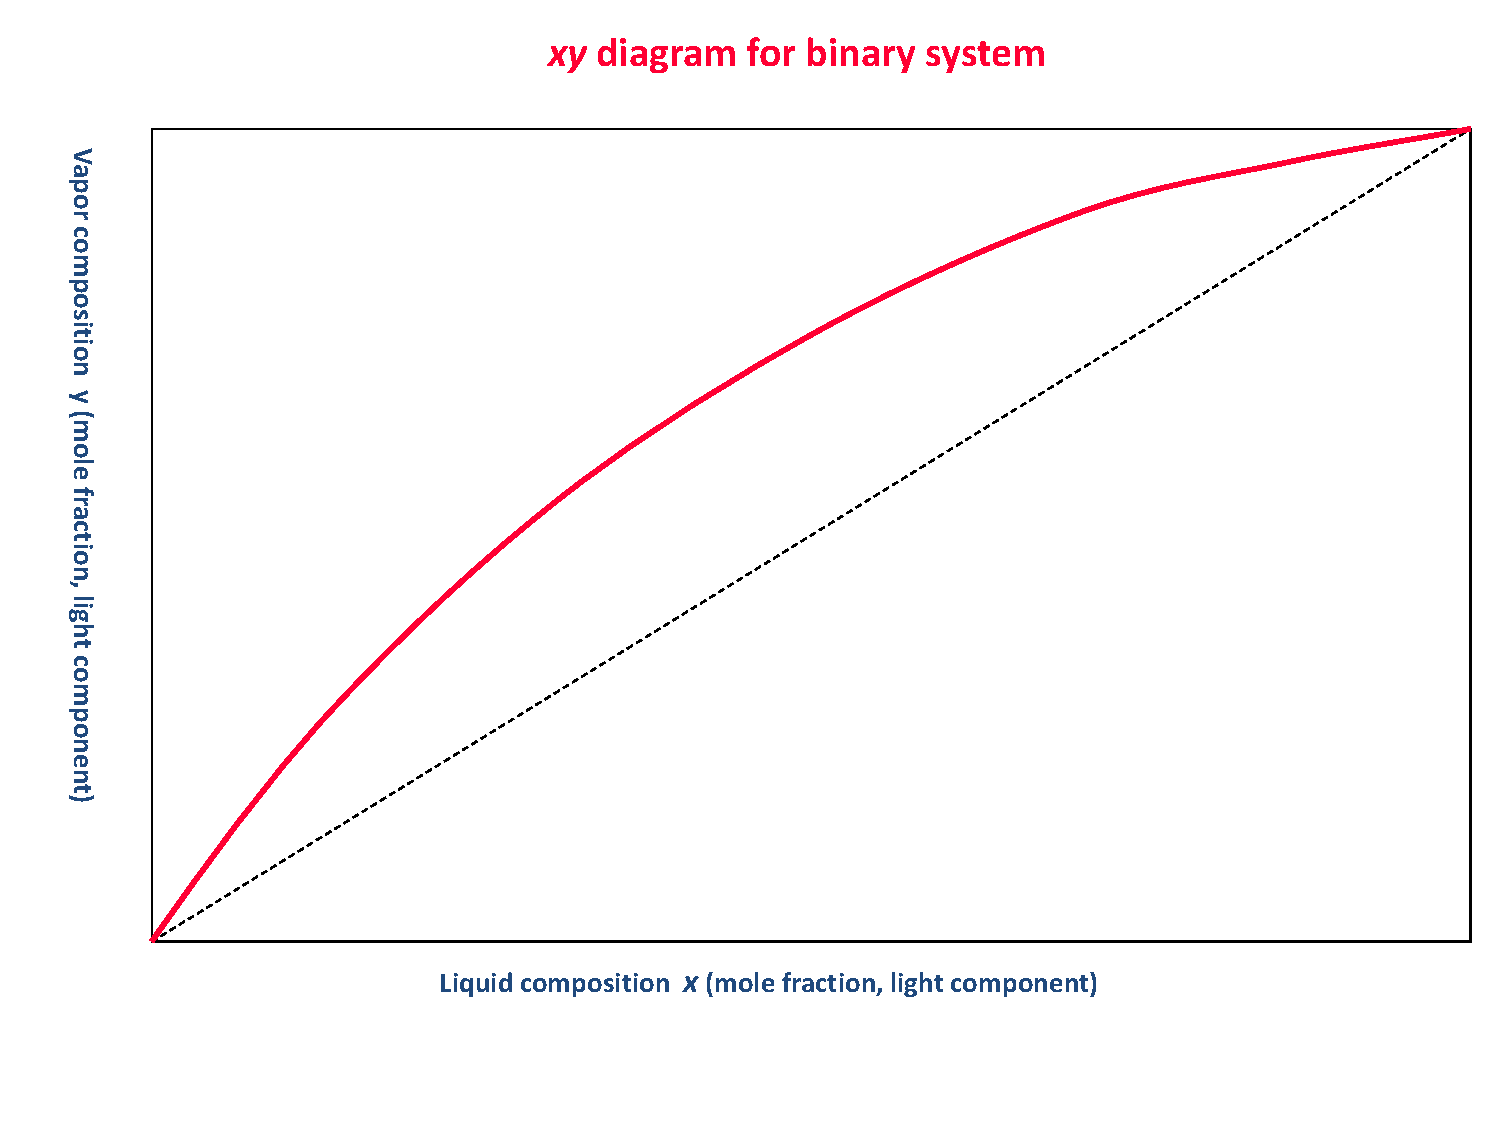
\includegraphics[width=5.5cm,height=4.cm,clip]{./../Pics/VLE_xy_DiagramIdeal}} \hspace{1cm}
           \visible<2->{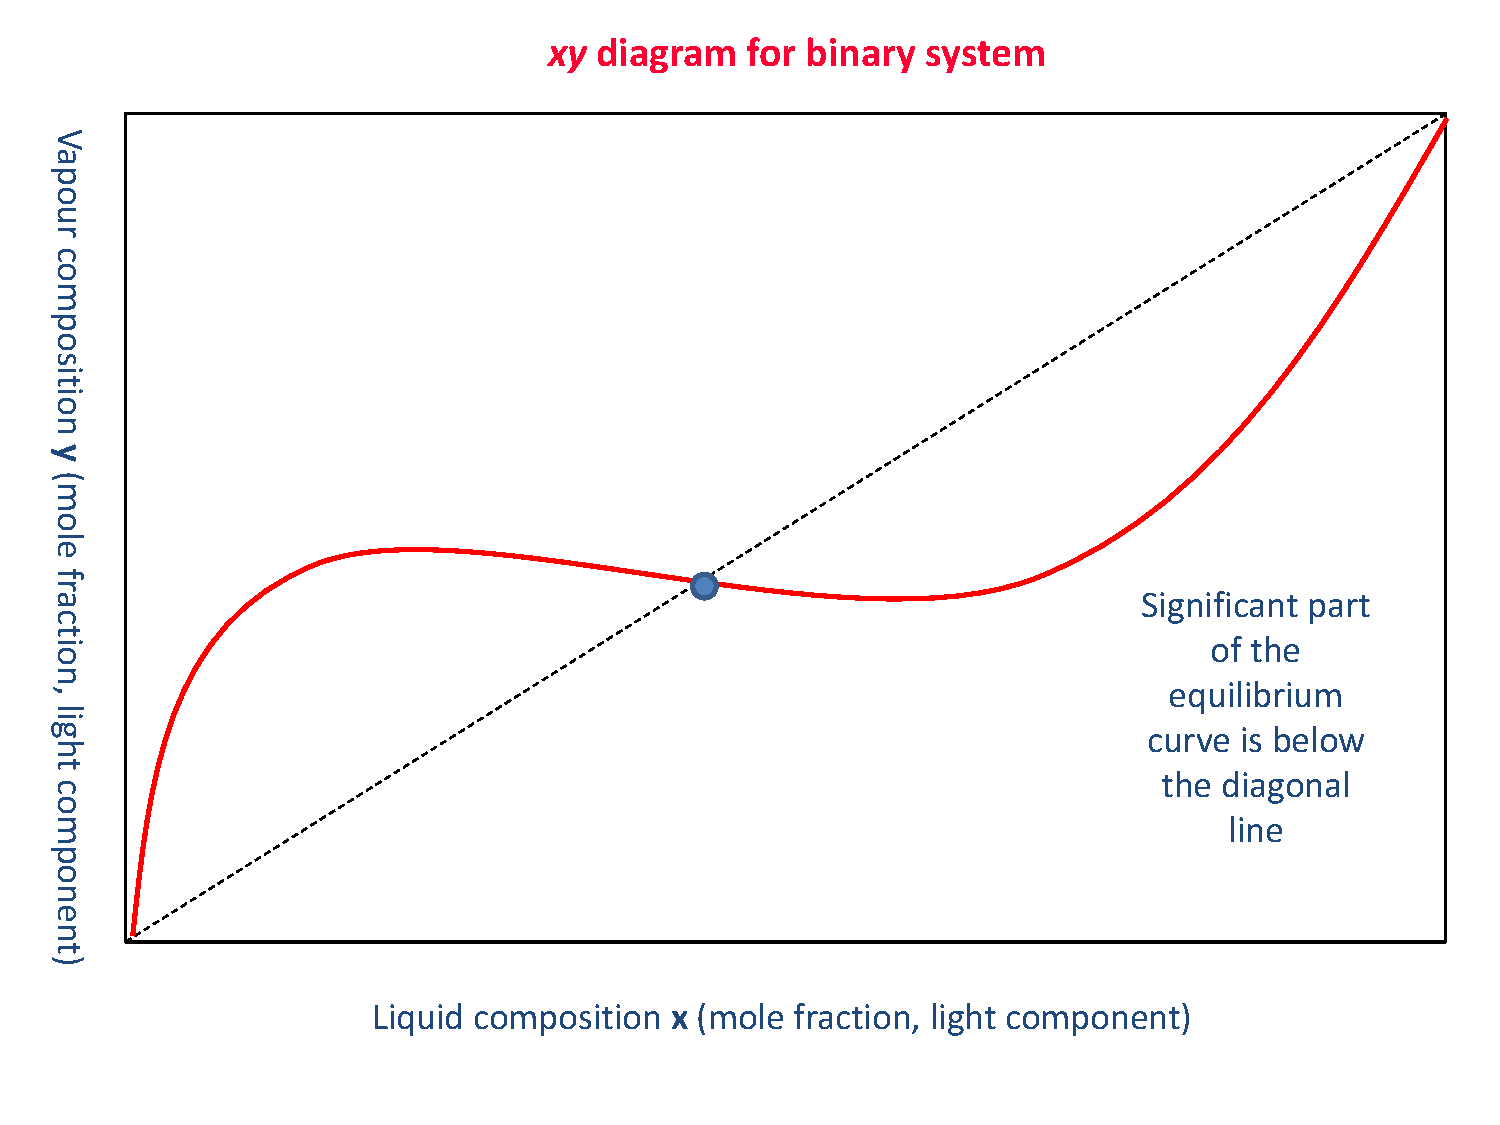
\includegraphics[width=5.5cm,height=4.cm,clip]{./../Pics/VLE_xy_DiagramNonIdeal1}}}
  \vspace{-0.2cm}
  \hbox{\hspace{4cm}
        \visible<3->{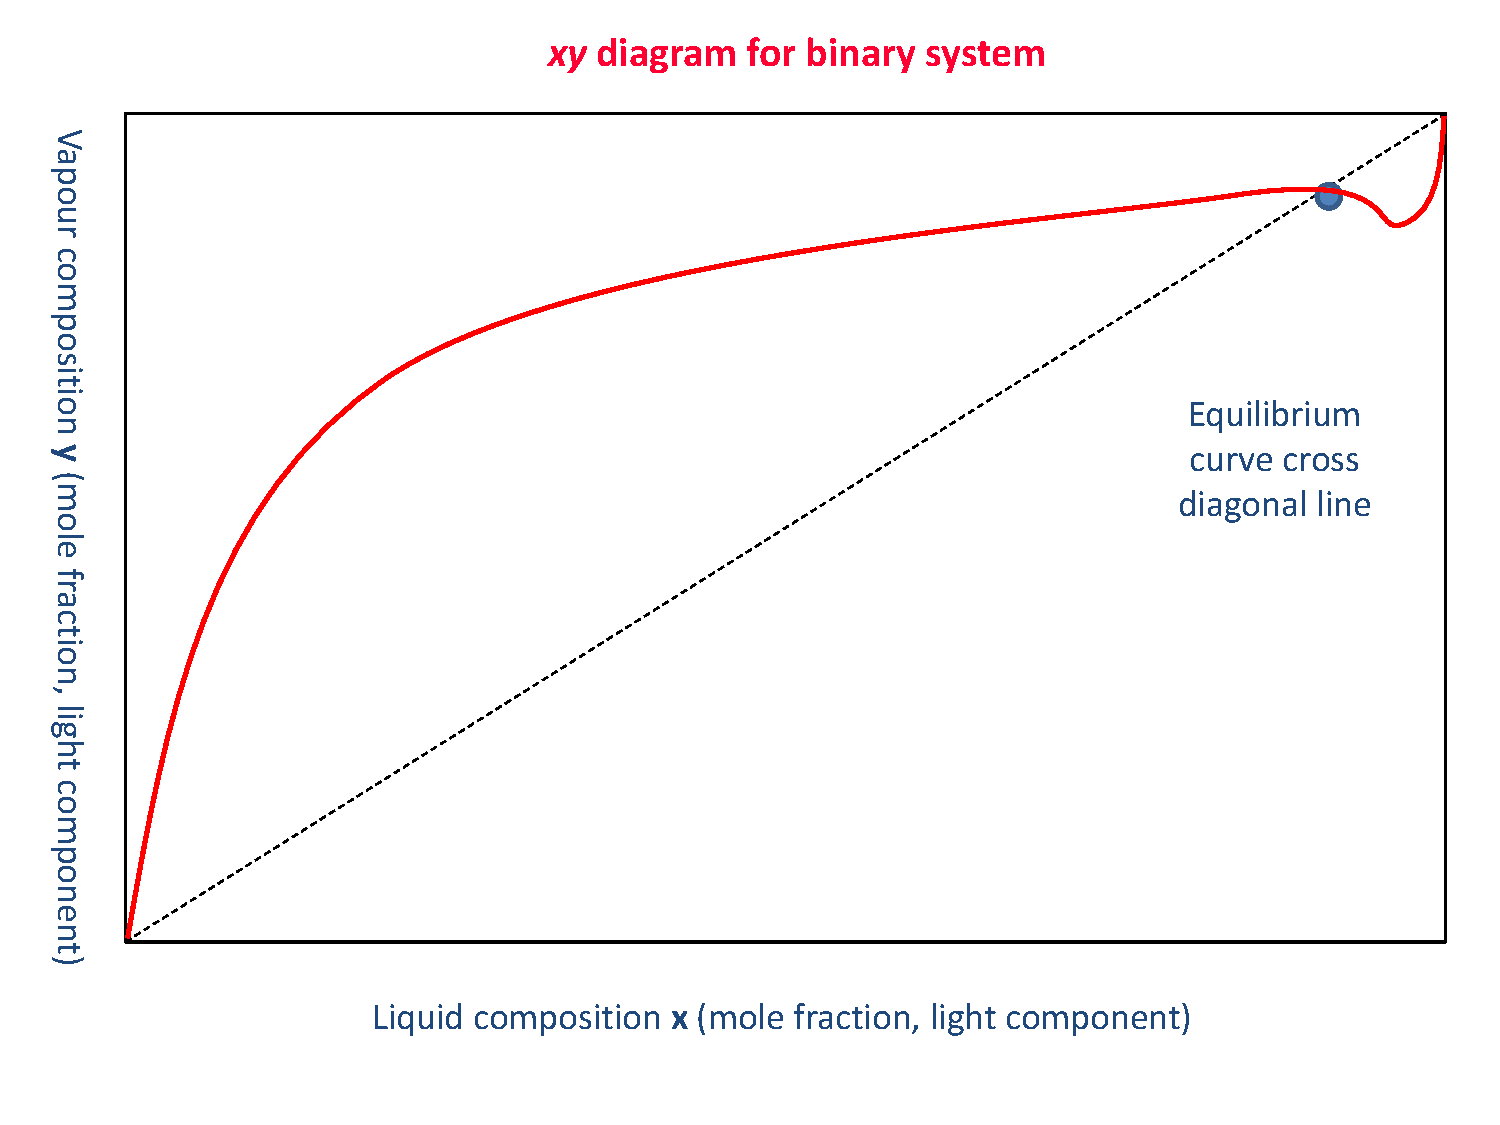
\includegraphics[width=5.5cm,height=4.cm,clip]{./../Pics/VLE_xy_DiagramNonIdeal2}}}
  }
\end{frame}
\normalsize


%%%
%%% SUBSECTION
%%%
\subsection{Simple Models}

%%%
%%% Slide
%%%
\begin{frame}
  \frametitle{General Remarks}
  \begin{enumerate}
      \item<1-> \textcolor{blue}{VLE models} aim for mathematical descriptions of the PVT behaviour of mixtures at equilibrium conditions:
         \begin{enumerate}
            \item<1-> Prediction of \textcolor{blue}{vapour and liquid compositions} at given $T$ and $P$;
            \item<1-> Basis for process modelling.
         \end{enumerate}
      \item<2-> Two simple models:
         \begin{enumerate}
            \item<2-> \textcolor{blue}{Raoult's law};
            \item<2-> \textcolor{blue}{Henry's law}.
         \end{enumerate}
  \end{enumerate}
\end{frame}

%%%
%%% Slide
%%%
\begin{frame}
  \frametitle{Raoult's Law}
  \begin{enumerate}
      \item<1-> Main assumptions:
         \begin{enumerate}
             \item<1-> \textcolor{blue}{vapour phase} behaves as an {\bf ideal gas} $\Longrightarrow$ low to moderate pressures;
             \item<1-> \textcolor{blue}{liquid phase} is an {\bf ideal solution}.
         \end{enumerate}
         \visible<2->{\begin{block}{Raoult's Law}
              \begin{displaymath}
                  \textcolor{blue}{ P_{i}= y_{i}P = x_{i} P_{i}^{\text{sat}}\left(T\right)}\;\;\;\;\textcolor{blue}{\forall i\in\left\{1,2,\cdots,\mathcal{C}\right\}}
              \end{displaymath}
         \end{block}
         where $P_{i}=y_{i}P$ is the {\bf partial pressure} of species {\it i} in the vapour phase.}
      \item<2-> This equation indicates that the partial pressure of a component in an ideal solution is equal to the product of the species mole fraction and its vapour pressure (of the pure component);
      \item<3-> Two major constraints:
         \begin{enumerate}
             \item<2-> Mass balance of both phases: $\sum\limits_{i=1}^{\mathcal{C}} x_{i} = 1$ and $\sum\limits_{i=1}^{\mathcal{C}} y_{i} = 1$
             \item<2-> {\bf Ideal solution:} \textcolor{blue}{$x_{i}\rightarrow 1$}. Also species {\bf must} be chemically similar (i.e., size, same chemical nature, e.g., isomers such as ortho-, meta-, and para-xylene) 
         \end{enumerate}
  \end{enumerate}
\end{frame}


%%%
%%% Slide
%%%
\begin{frame}
  \frametitle{Raoult's Law: Ideal gas mixture properties}
  \begin{enumerate}
      \item<1-> Dalton's Law: \textcolor{blue}{$P=\sum\limits_{i=1}^{\mathcal{C}}P_{i}=\sum\limits_{i=1}^{\mathcal{C}}y_{i}P$}
      \item<2-> Amagat's Law: \textcolor{blue}{$V^{t}=\sum\limits_{i=1}^{\mathcal{C}}V_{i}^{t} = \sum\limits_{i=1}^{\mathcal{C}} y_{i}V^{t}$}
      \item<3-> Kay's rule: pseudo-critical pressure \textcolor{blue}{$\left(T_{c}^{t}=\sum\limits_{i=1}^{\mathcal{C}}y_{i}T_{c,i}\right)$} and temperature \textcolor{blue}{$\left(T_{c}^{t}=\sum\limits_{i=1}^{\mathcal{C}}y_{i}T_{c,i}\right)$}. 
  \end{enumerate}
\end{frame}

%%%
%%% Slide
%%%
\begin{frame}
  \frametitle{Raoult's Law: Dew and Bubble Point Calculations}
  \begin{description}
      \item[Dew Point:]<2->: Calculate, 
           \begin{enumerate}
               \item<2-> $\textcolor{blue}{\bf x_{i}}$ and \textcolor{blue}{$P$}, given $y_{i}$ and $T$;
               \item<2-> $\textcolor{blue}{\bf x_{i}}$ and \textcolor{blue}{$T$}, given $y_{i}$ and $P$;
           \end{enumerate}
      \item[Bubble Point:]<3-> Calculate, 
           \begin{enumerate}
               \item<3-> $\textcolor{blue}{\bf y_{i}}$ and \textcolor{blue}{$P$}, given $x_{i}$ and $T$;
               \item<3-> $\textcolor{blue}{\bf y_{i}}$ and \textcolor{blue}{$T$}, given $x_{i}$ and $P$.
           \end{enumerate}
  \end{description}
\end{frame}

\begin{frame}
  \frametitle{Generalised Relation for VLE in Ideal Mixtures}
  \begin{enumerate}
      \item<1-> Raoult's law is a particular case of a more general relation involving \textcolor{blue}{vapour-liquid mixtures} (that we will see with more details on Module 5),
           \visible<2->{\begin{displaymath}
              f_{i}^{\left(L\right)}\left(T,P,\underline{x}\right) = f_{i}^{\left(V\right)}\left(T,P,\underline{y}\right)
           \end{displaymath}
           where $\underline{x}$ and $\underline{y}$ represent the array of compositions in the liquid and vapour phases, respectively.}
      \item<3-> For low-pressure VLE,
           \visible<3->{\begin{displaymath}
               \textcolor{blue}{y_{i}P=x_{i}\gamma_{i}P_{i}^{\text{sat}}}
           \end{displaymath}}
      \item<4-> The activity  coefficient of species $i$, $\gamma_{i}$, is a thermodynamic property that indicates $\lq$how much a solution will deviate from the ideal solution';
      \item<4-> For an ideal solution, $\gamma_{i}=1$, and the equation above becomes the Raoult's law.  
  \end{enumerate}
\end{frame}

%%%
%%% Slide
%%%
\begin{frame}
  \frametitle{Henry's Law}
  \begin{enumerate}
      \item<1-> Raoult's law requires vapour pressure data $\left(\text{i.e., }P_{i}^{\text{sat}}\right)$, thus:
        \begin{enumerate}
            \item<1-> It is not applicable if $T\geq T_{c,i}$;
            \item<1-> Does not take into account gasses dissolved in the liquid.
        \end{enumerate}
      \item<2-> Henry's law:
         \visible<2->{\begin{displaymath}
             \textcolor{blue}{y_{i}P = x_{i}\mathcal{H}_{i}}\;\;\;\;\forall i\in\left\{1,2,\cdots,\mathcal{C}\right\}
         \end{displaymath}}
  \end{enumerate}
  \visible<2->{
 \begin{table}
  \begin{center}
    \begin{tabular}{l r || l r }
      \hline
       {\bf Gas}    &  ${\bf \mathcal{H}\text{ (bar)}}$ & {\bf Gas}    &  ${\bf \mathcal{H}\text{ (bar)}}$ \\
      \hline
         Acetylene  &   1350                            & He           &  126600 \\
         Air        &   72950                           & H$_{2}$      &  71600  \\
         CO$_{2}$    & 1670                              & H$_{2}$S     & 550 \\
         CO         &  54600                            &  CH$_{4}$    &  41850 \\
         C$_{2}$H$_{6}$ & 30600                          &  N$_{2}$     & 87650  \\
         Ethylene  & 11550                              & O$_{2}$      & 44380 \\
      \hline
    \end{tabular}
    \caption{Henry's constant for gases dissolved in water at 25$^{\circ}$C.}
  \end{center}
\end{table}}
\end{frame}


%%%
%%% Slide
%%%
\begin{frame}
  \frametitle{K-Value Correlations}
  \begin{columns}
     \begin{column}[l]{0.5\linewidth}
        \begin{enumerate}
           \item<1-> Equilibrium ratio, $K_{i}$
               \visible<1->{\begin{displaymath}
                  K_{i} = \frc{y_{i}}{x_{i}}
               \end{displaymath}}
           \item<2-> With Raoult's law:
               \visible<2->{\begin{displaymath}
                  K_{i} = \frc{P_{i}^{\text{sat}}}{P}
               \end{displaymath}}
           \item<3-> With modified Raoult's law:
               \visible<3->{\begin{displaymath}
                  K_{i} = \frc{\gamma_{i}P_{i}^{\text{sat}}}{P}
               \end{displaymath}}
        \end{enumerate}
     \end{column}
     \begin{column}[l]{0.5\linewidth}
        \begin{center}
            \hspace{-.8cm}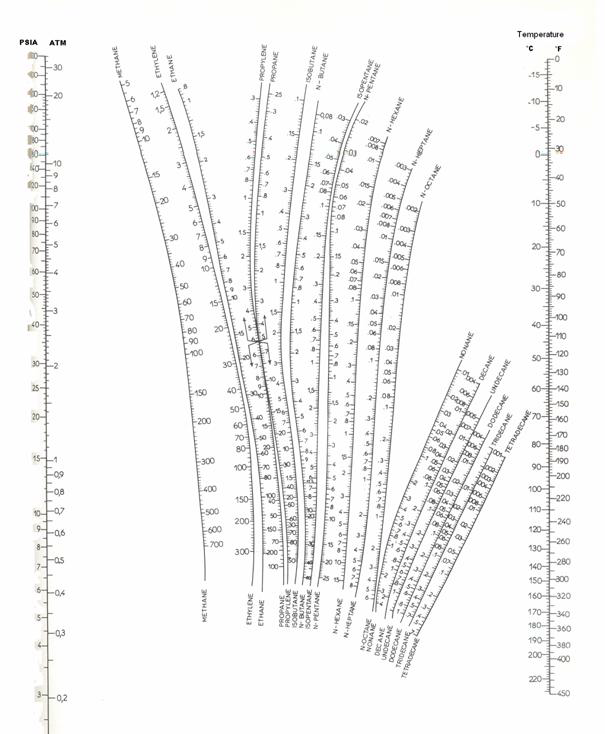
\includegraphics[width=6.1cm,clip]{./../Pics/02_07_fig_02.png}
        \end{center}
     \end{column}
   \end{columns}
\end{frame}


%%%
%%% Slide
%%%
\begin{frame}
  \frametitle{Flash Calculations}
  \begin{columns}
     \begin{column}[c]{0.5\linewidth}
       \visible<3->{\hspace{-1cm}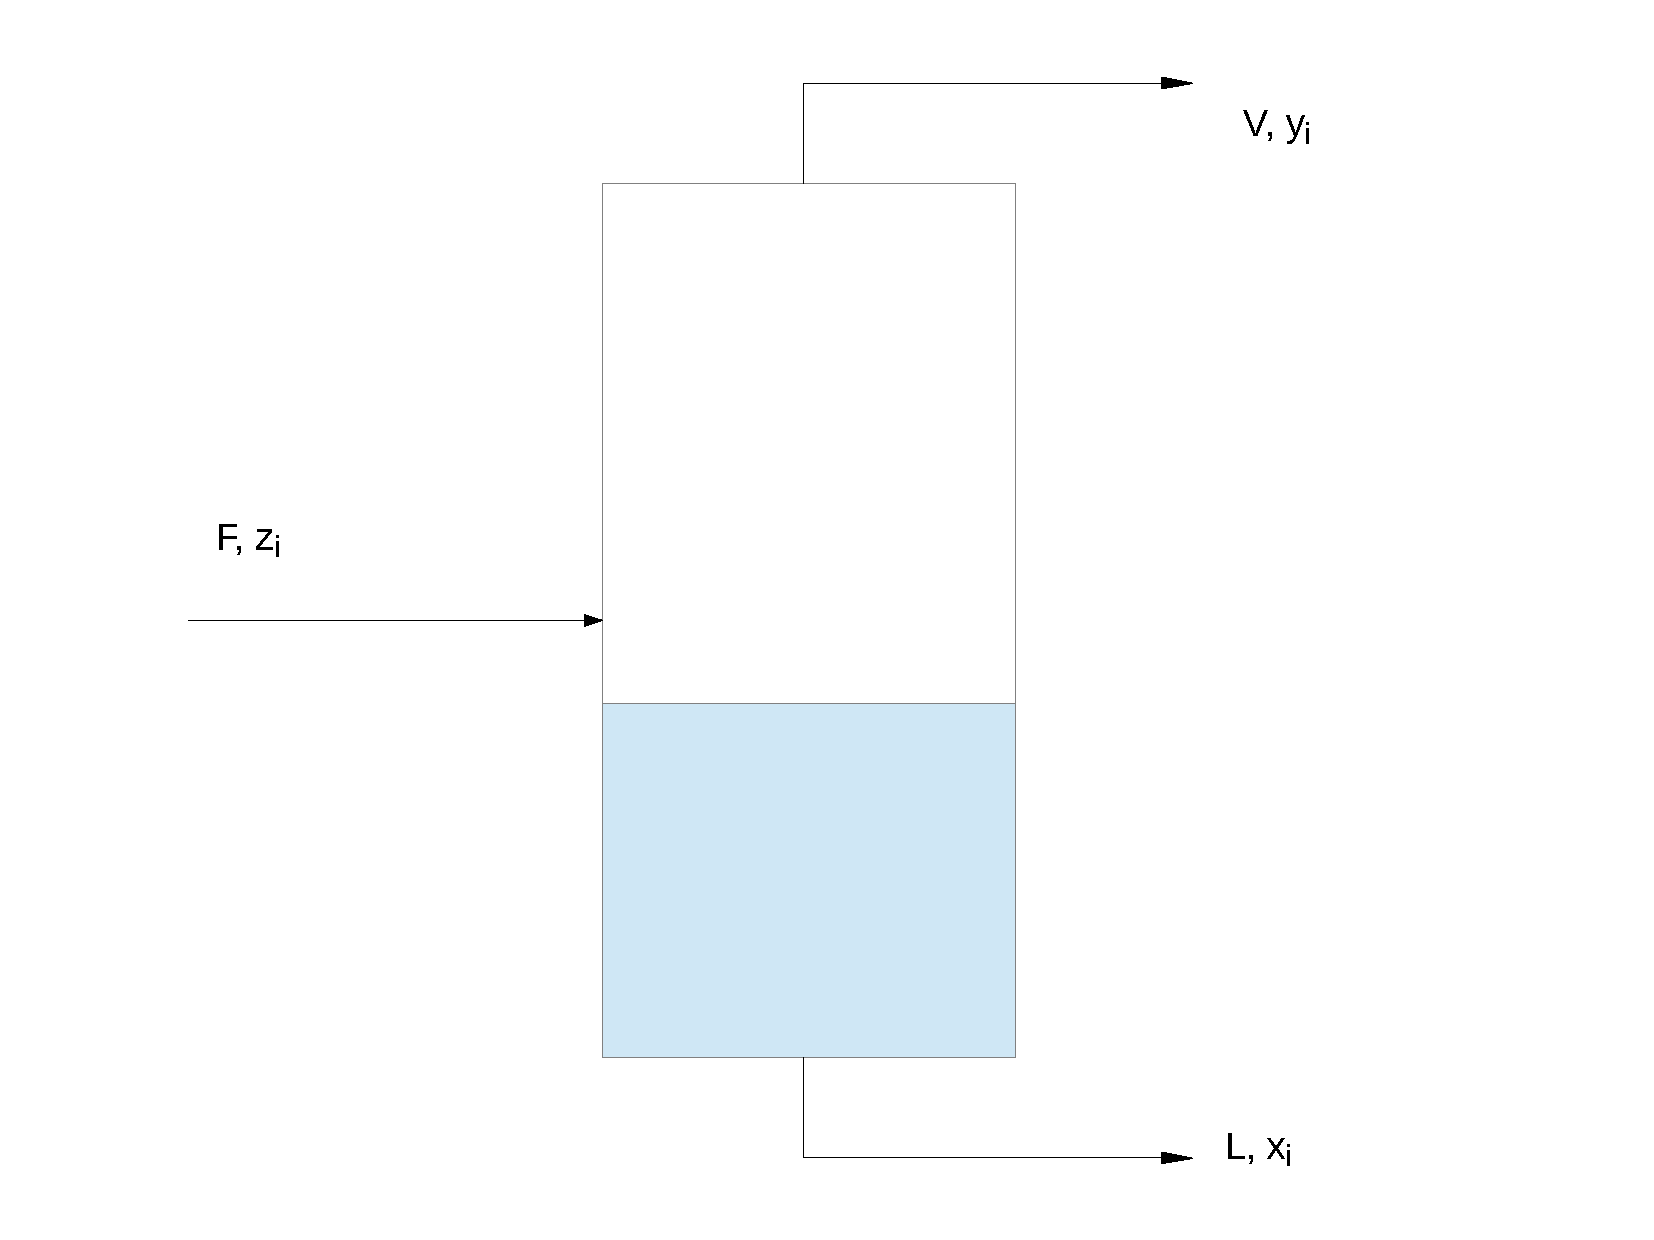
\includegraphics[width=1.3\linewidth,clip]{./../Pics/Flash_VLE}}
     \end{column}
     \begin{column}[l]{0.5\linewidth}
        \begin{enumerate}
           \item<1-> If a fluid mixture is at liquid state with pressure larger than the associated bubble point pressure; % $\left(\text{i.e., }P \leq P_{\text{BP}}\right)$;
           \item<2-> Part of the fluid evaporates \textcolor{blue}{(or {\it flashes})} when the pressure is reduced leading to a two-phase system -- vapour and liquid in equilibrium;
            \item<3-> This phenomenon is often called \textcolor{blue}{\it flash} and is the most important application of VLE;
            \item<4-> Thus, a feeding stream $F$ with overall composition $z_{i}$ is separated into vapour ($V$) and liquid ($L$) streams with compositions $y_{i}$ and $x_{i}$, respectively. 
        \end{enumerate}
     \end{column}
   \end{columns}
\end{frame}


\section{Summary}

%%%
%%% Slide
%%%
%\scriptsize
\begin{frame}
 \frametitle{Summary}
   \begin{enumerate}[(i)]
     \item Stability conditions/criteria;
     \item Phase rule and Duhem's theorem;
     \item Qualitative analysis of VLE -- efficient use of graphical representation of $P$, $T$ and composition of species;
     \item Introduction to generalised relation for VLE in non-ideal mixtures;
     \item Raoult and Henry's laws; 
     \item Industrial application for VLE: Flash problem.
   \end{enumerate}
\end{frame}


\end{document}
 
